%!TEX root = ../../main.tex


\begin{figure}[p]
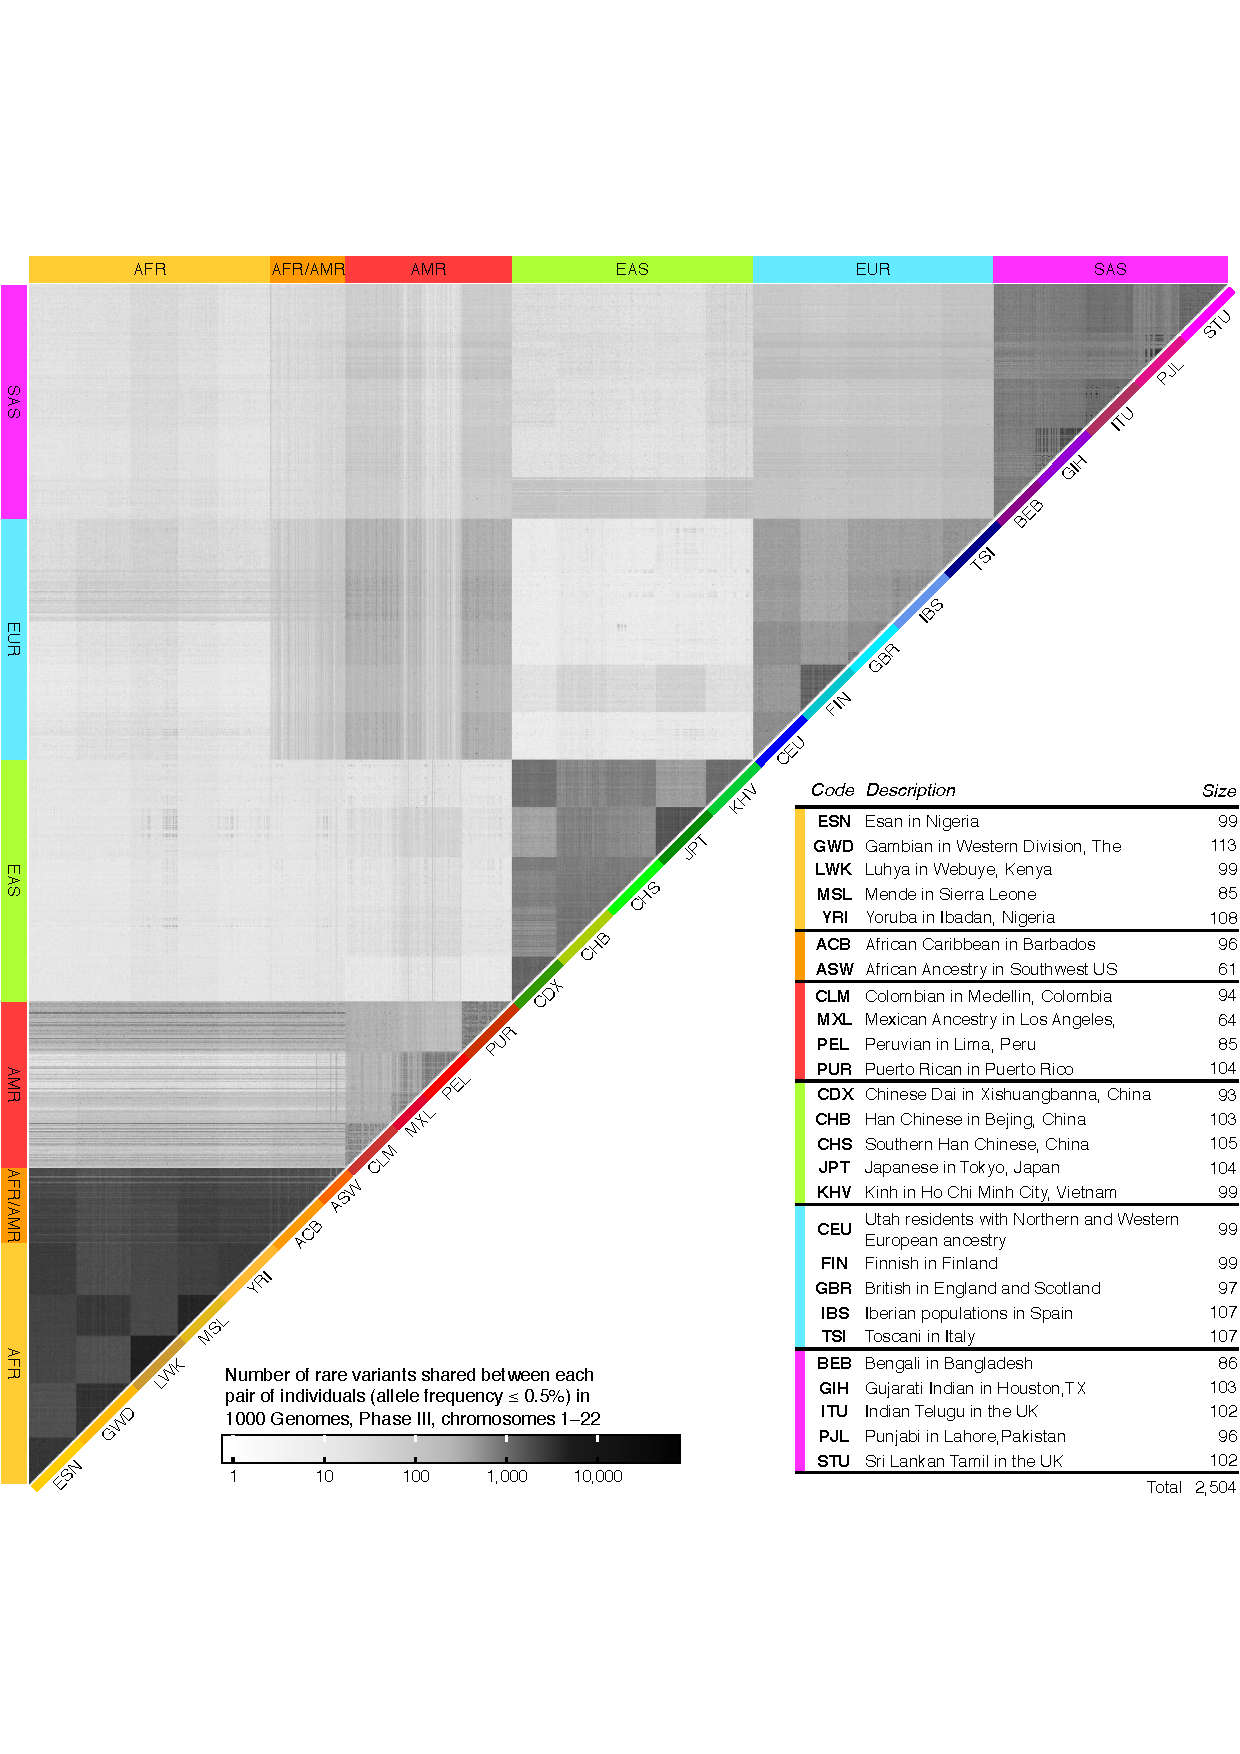
\includegraphics[width=\textwidth]{./img/ch3/popstruct_1kg}
\Caption{Rare variant sharing in the 1000 Genomes dataset}
{The plot shows the upper triangle of a pairwise sharing matrix in which the number of variants shared in each pair of individuals is indicated by tones of grey (log-scaled), ranging from \emph{light} (low number) to \emph{dark} (high number); see legend.
Pairwise rare variant sharing was determined for all shared alleles observed at  frequency ${\leq 0.5\%}$, across chromosomes 1--22, and in each pair of the \n{2504} individuals present in the final release dataset of the \glsentrylong{1kg} Phase~\rom{3}.
The dataset comprises sample data from \n{6} continental populations (or \emph{super-populations}) which are further subdivided in \n{26}~populations of different ethnic background.
Each group is abbreviated using a \n{3}-letter code.
The \n{6} continental populations are defined as follows;
African~(AFR), African-American~(AFR/AMR), American~(AMR), East~Asian~(EAS), European~(EUR), and South~Asian~(SAS).
The table in the lower right corner shows the code and description of each  population sample, as well as the number of individuals in each group.}
{fig:popstruct_1kg}
\end{figure}
